
\begin{figure}
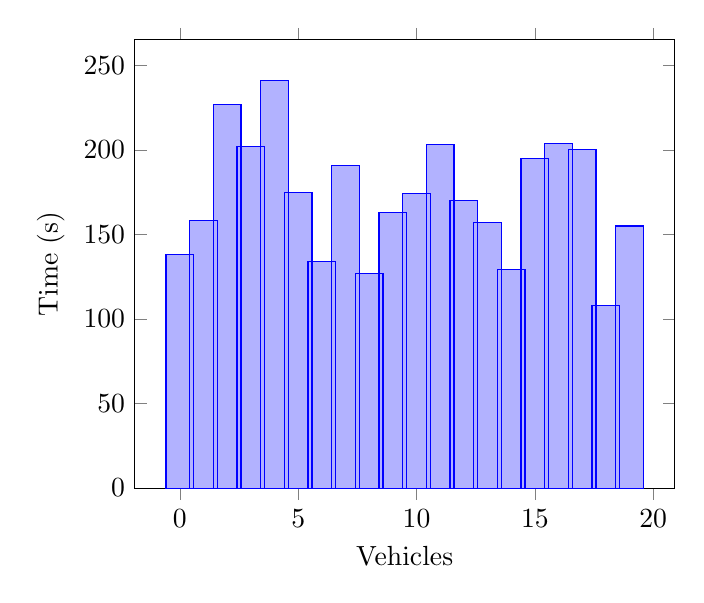
\begin{tikzpicture}
\begin{axis}[
legend style={anchor=west},
xlabel=Vehicles,
ylabel=Time (s),
ymin=0,
ybar,
]
\addplot coordinates {
(0, 138)
(1, 158)
(2, 227)
(3, 202)
(4, 241)
(5, 175)
(6, 134)
(7, 191)
(8, 127)
(9, 163)
(10, 174)
(11, 203)
(12, 170)
(13, 157)
(14, 129)
(15, 195)
(16, 204)
(17, 200)
(18, 108)
(19, 155)
};

\end{axis}
\end{tikzpicture}
\label{tik:100:2_O, 2_O.-60, 4_S, 5_S, 5_S.-30, 7_S, 7_S.-25, 11_S, 11_S.-50, 13_S, 15_N, 17_S, 17_S.-60, 20_O, 21_O}
\caption{100 percent diving with GSC on route $2_O, 2_O.-60, 4_S, 5_S, 5_S.-30, 7_S, 7_S.-25, 11_S, 11_S.-50, 13_S, 15_N, 17_S, 17_S.-60, 20_O, 21_O$}
\end{figure}
